\documentclass{article}
%First, we define our document class. Article is the most flexible, but other types include reports, books and even slides (using either slides or beamer)

%The document we just used - "A Basic Tex Document.tex" - shows us the bare minimum we need to make something in LaTeX.

%Let's try LaTeX Exercise 1!

%For more complex documents, we'll want to add packages containing extra useful features. We usually try to group these all together:
\usepackage{soul} %highlighting
\usepackage[toc,page]{appendix} %lets us make an appendix
\usepackage{enumitem} %this package lets us customize list types
\usepackage{amsmath} %this package will let us use the align environment, and generally make our equations prettier
\usepackage{hyperref} %lets you embed hyperlinks into your document
\usepackage{graphicx} %a great package for adding figueres 
\usepackage{caption} %for making subcaptions in figures
\usepackage{subcaption} %for making subcaptions in figures
\usepackage{parskip}

%\renewcommand{\thesection}{\Roman{section}}

%We can add our title info here:
\title{\LaTeX\ Fundamentals: Part 1}
\date{Fall 2018} % without this, LaTeX will call today's date into the title
\author{Isabelle M. Cohen \\ DLab}

\begin{document}

%First, we call our title

\maketitle
\clearpage 
%Making a table of contents is super easy
\tableofcontents
\clearpage
%Next, we create a section, with the command \section. We give the section a title inside "{" symbols after the word section. 

\section{Welcome to \LaTeX!}\label{welcome}

\LaTeX\  is a document creation software which uses plain text with what are called ``mark-up tagging conventions.'' We are in Section \ref{welcome}.

%Notice how the things we write after ``%'' symbols don't show up in the main document?

%Also note that to get quotation marks, we type `` before the word and '' after.

%Next, we'll use the enumerate environment; this lets us make a numbered list. 
\LaTeX\  has all kinds of useful features:
\begin{enumerate}
	\item It right and left-justifies your text, in a way that looks much better than Microsoft Word. 
	
	Doesn't it look good?
	\item It's great for writing lengthy equations
	\item It makes it easy to integrate your bibliography into your document, using what's called BibTex
	\item It's easy to export statistical analysis from Stata or R directly into a convenient LaTeX format
\end{enumerate}

Overall, while \LaTeX\  might not be the easiest program to start using, it can help make your life easier, and your work look more professional.

The basic way that \LaTeX\ works is that you write code and text together in a writing environment (like TexStudio, but it can also be simpler), then compile your code. The compiling reads the code into the text, and produces a formatted document, typically a .pdf (but we can also make a .ps or .dvi file). The text editor and the distribution (what does the compiling) are often bundled together, like in TexStudio.

In this workshop, we discuss basic set-up, lists, math mode, figures and other uses for \LaTeX.

\section{Basic set-up}

A \LaTeX\ document contains all kind of stuff you never see. 

\subsection{Preamble}

In our preamble, we set our document type and call the packages we want! We can also add in custom commands or shortcuts, format page headers/footers and numbers, and do all kinds of other overall document formatting.

\subsection{Title}

We can also use the preamble to make our title. The default way is to specify your title, author and date information in the preamble, then use the maketitle command in the body of the document. 

\subsubsection{So cool}

\section{Lists}

There are a lot of types of list in \LaTeX! Lists are not only useful, but they'll also help introduce us to some of the principles of formatting text in \LaTeX. 

To make a list, we set what's called an \emph{environment}. That means we need to begin the environment (which requires calling it by name), fill it with content, then end it (again by name). The list below is made with the enumerate environment; the one in Section \ref{welcome} is made with the itemize environment.

%Notice how we wrote \ref{welcome} instead of 1 in the sentence above? When we made our section title for section 1, we labeled it welcome using \label{welcome}. Now, instead of typing our the section number - which could change as we work on the document - we can just use the \ref command. This also creates a hyperlink within the document, which would take us back to the first section.

\begin{enumerate}[label=\Alph*.]
	\item We can do simple bullet points with the itemize environment
	\item We can do numbers with the enumerate default environment
	\item By using the enumitem package, we also get more exciting options, like the alphabet, which uses the phrase \begin{verbatim} [label=\alph*.] \end{verbatim} after we begin the environment
	
%Notice how we use the verbatim environment inside the list? This lets us display the code as is, without LaTeX interpreting it. 

%Isn't it cool that we can write comments right in the middle of our code?

	\item We could even use roman numerals with the roman option. 
	\begin{enumerate}[label=\Roman*]
		\item That
		\item looks
		\item good!
	\end{enumerate}
	\item We can choose whether or not to specify periods, parenthesis, etc.; for example, with \begin{verbatim} [label=(\roman*)] \end{verbatim}
	\begin{enumerate}[label=(\roman*)]
		\item Then
		\item we
		\item would
		\item get
		\item this
	\end{enumerate}
\end{enumerate}
	
\begin{itemize}
	\item Lists
	\item can
	\item also
	\item look
	\item like
	\item this
\end{itemize}

%It's your turn to practice, using LaTeX Exercise 2.

\section{Math Mode}

Math mode is where \LaTeX\ really shines. Math mode lets you add mathematical symbols and equations in your document. Let's say you want to write an equation about y, or $y$, and f(x), or $f(x)$.

%Notice how we use the $ symbol to turn y and f(x) into terms that look more like an equation! When we surround something by a pair of $s in text, that creates math mode on the line.

We might want the equation on its own line. One way to do this is to use a slash, $\backslash$, and a bracket, [, one at the beginning, and one at the end.

\[
y=f(x)
\]

Another way is to use the align environment, which gives our equation a number.
\begin{align}
y=f(x)
\end{align}

We can also turn off the equation number by using align* instead.
\begin{align*}
y=f(x)
\end{align*}

All three equations look almost exactly the same. No matter how you enter math mode, the equations look much the same. There are various other environments that also let you use math mode in its own paragraph, including \$\$ (not very popular), the displaymath environment, the equation environment, and the gather (or gather*) environment.

Notice how it isn't very easy to put a $\backslash$ in your text. Here's what happens when we try to do it: \

Nothing happens! Instead, we actually used math mode in the line, with the word backslash. This is the main way we write mathematical symbols, whether in or our of math mode. For example, to get the Greek alphabet:
\[ 
\alpha, \beta, \gamma, \delta, \epsilon, \zeta, \eta, \theta, \iota, \kappa, \lambda, \mu, \nu, \xi, \pi, \rho, \sigma, \tau, \upsilon, \phi, \chi, \psi, \omega 
\]

\[
\lambda, \Lambda
\]

which is just like writing alpha, beta, gamma, delta, epsilon, zeta, eta, theta, etc. with $\backslash$ before them inside math mode. 

%Omicron is missing; this is because it basically just looks like o.

\LaTeX\ also allows us to write more complicated math, for example including square roots (sqrt) and superscripts (\^{}).
%Notice that getting the carrot is really tricky. We used a backslash before it, and two brackets after.
\[
y = \sqrt{x + 1} + x + x^2
\]

We can also use subscripts, parenthesis, brackets, square brackets, and even fractions.
\[
y = \frac{(x^3+x^2)}{x+4}
\]

We can also write simple integrals:
\[
\int_0^2x^2 - 1 dx
\]
or derivatives of trigonometric functions:
\[
\frac{d}{dx}(\sinh(u))=\cosh(u)\frac{du}{dx}
\]

Let's dig into subscripts and superscripts. We can write a squared variable as easily as $x^2$, or use a subscript the same way with $x_2$. For more complex subscripts, we would just place brackets around the content of the superscript ($x^{2y}$) or subscript ($x_{ijk}$). We can even include both: $x^{2y}_{ijk}$

It's also worth discussing parenthesis, brackets and curly brackets further.These may seem simple, but they can make a huge difference in the readability of your equation.

Without customization, you may find your parenthesis the wrong size:
\[
(\frac{2x} % numerator
{y}) % denominator 
\]

This is pretty easy to fix by putting a $\backslash$ left before the parenthesis and a $\backslash$ right after:
\[
\left(\frac{2x}{y}\right)
\]

The left and right commands will automatically resize parenthesis or brackets no matter how large:
\[
\left[\frac{\left(\frac{2x}{y}\right)}{z}\right]
\]

%Just make sure you don't forget to close your parenthesis!

To add in curly brackets, just use $\backslash$ before the brackets, even without resizing.

\[
\left[\frac{\left(\frac{2\{x+1\}}{y}\right)}{z}\right]
\]

To make them scalable, we just use $\backslash$ left $\backslash$ bracket to start, and $\backslash$ right $\backslash$ bracket to close.

\[
\left\{\frac{2x}{y}\right\}
\]

%Let's make math mode magic using LaTeX Exercise 3!

If we want to write more complex sets of equations, we could use the align package. We can use $\backslash\backslash$ to mark the end of the line, and \& to indicate where the equals signs should line up.

%This is the same way we'll demarcate columns and rows in tables in the very next section.

\begin{align}
\frac{\partial x_i(\mathbf{p},w)}{\partial p_j}&= \frac{\partial h_i(\mathbf{p},u)}{\partial p_j}-\frac{\partial x_i(\mathbf{p},w)}{\partial w}x_j(\mathbf{p},w) \label{eq} \\
\epsilon_{p,ij} &=\epsilon^h_{p,ij} - \epsilon_{w,i}b_j
\end{align}

Equation \ref{eq} is above!

%Notice how we use the mathbf command to bold p and make it represent a vector.

Finally, what about matrices? For those, we like to use the array environment inside math mode, with scalable brackets:
\[ \left[
\begin{array}{ c c c }
1 & 2 \\
3 & 4 & 5
\end{array} \right]
\]

This array also gives us a little preview of Workshop 2; this structure closely resembles how \LaTeX sets up tables.


\section{Figures}

\LaTeX\ has a lot of different ways to insert and customize figures. We'll focus on the graphicx package.

The most basic use is just the command includegraphics, where we specify the file path (from our current folder) and the image name after the command. For this to work, the campanile image should be in the same folder as our \LaTeX\ document.

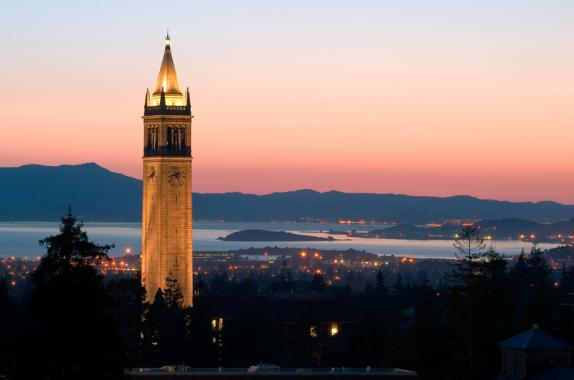
\includegraphics[width=\textwidth]{campanile.jpg}

In the command, we specified a width for the image - specifically, textwidth, which is roughly the width of the text. If we wanted it to be half as wide as the text, we could specify .5 textwidth, as below.

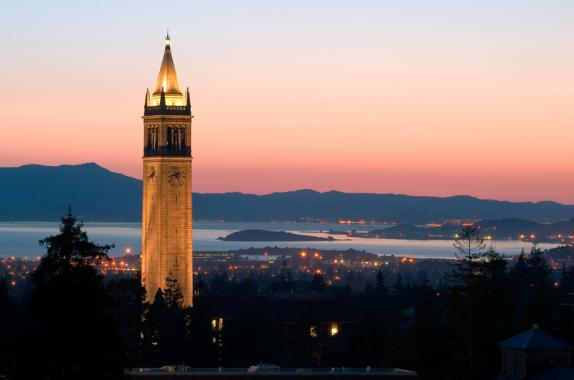
\includegraphics[width=.5\textwidth]{campanile.jpg}

Alternatively, we can fix the width or height to a certain size (1 cm, 2 cm, etc.) or adjust the scale of the image; instead of width, we type scale, and specify something relative to the original size of the image. We can also use the center environment again.

\begin{center}
	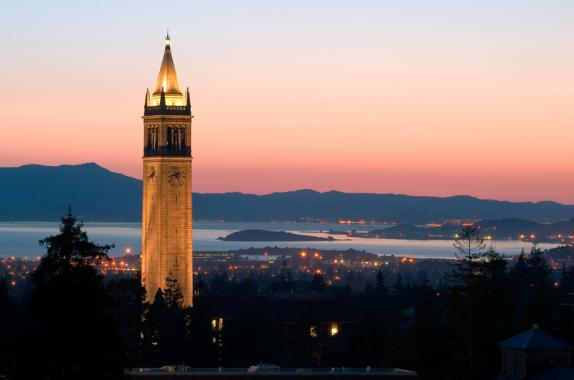
\includegraphics[scale=.5]{campanile.jpg}
\end{center}

The equivalent to the table environment is the figure environment. This will let us include a caption, fix the location of the figure, etc., and to use the centering option. We do this in Figure \ref{berkeley1} below. 

\begin{figure}[h!]
	\centering	
	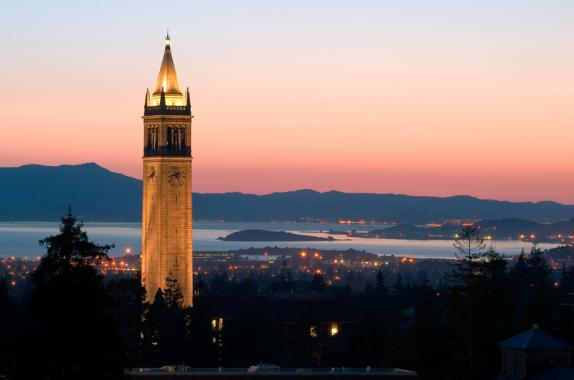
\includegraphics[width=.5\textwidth]{campanile.jpg}
	\caption{Berkeley at sunset}\label{berkeley1}
\end{figure}

If we want to include two images next to each other, we just include them in the same figure (with the width slightly less than half the text width).

\begin{figure}[h!]
	\centering	
	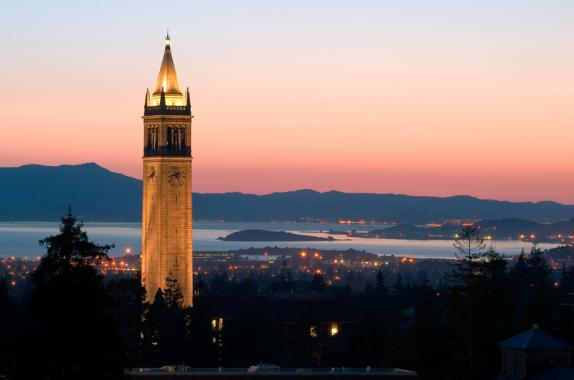
\includegraphics[width=.4\textwidth]{campanile.jpg}
	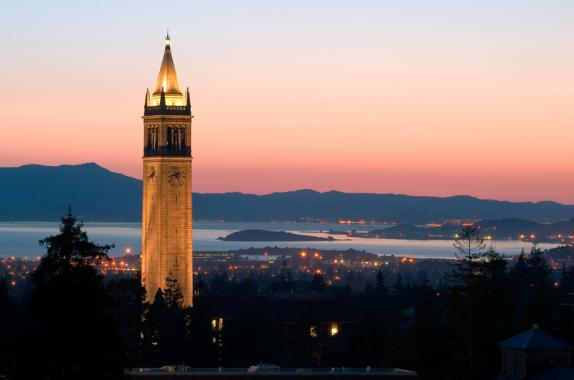
\includegraphics[width=.4\textwidth]{campanile.jpg}
	\caption{Berkeley at sunset - twice}
\end{figure}

Let's make things a little more complicated. Let's say we want to include two images in the same figure, but give them separate captions. There are a few ways to do that; one is below:

\begin{figure}[h!]
	\centering
	\begin{subfigure}[t]{1in}
		\centering
		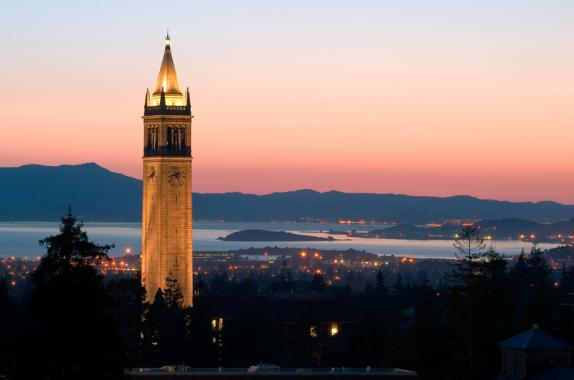
\includegraphics[width=1in]{campanile.jpg}	
		\caption{Berkeley 1}\label{fig:2a}			
	\end{subfigure}
	\begin{subfigure}[t]{1in}
		\centering
		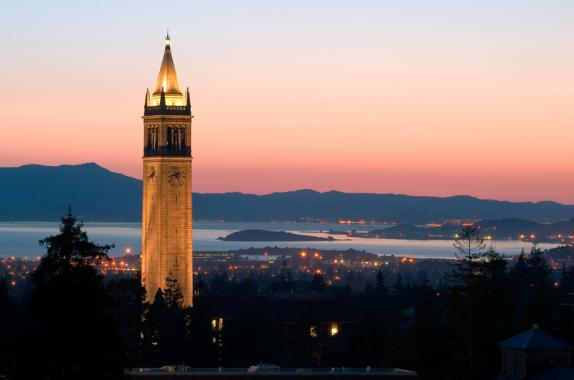
\includegraphics[width=1in]{campanile.jpg}
		\caption{Berkeley 2}\label{fig:2b}		
	\end{subfigure}
	\begin{subfigure}[t]{1in}
	\centering
	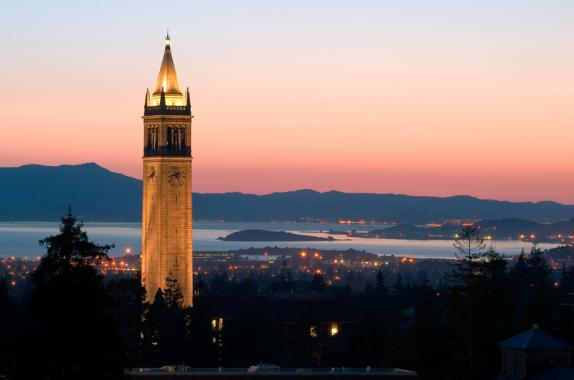
\includegraphics[width=1in]{campanile.jpg}	
	\caption{Berkeley 1}\label{fig:2a}			
	\end{subfigure}
	\begin{subfigure}[t]{1in}
		\centering
		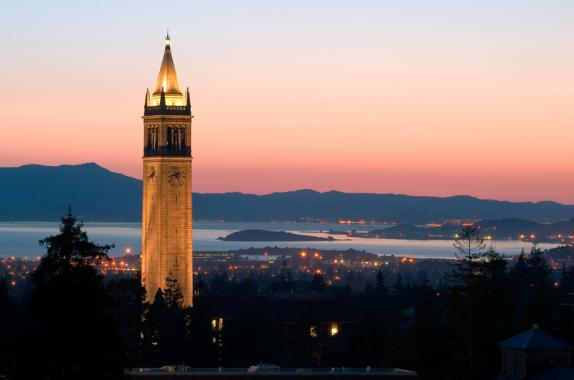
\includegraphics[width=1in]{campanile.jpg}
		\caption{Berkeley 2}\label{fig:2b}		
	\end{subfigure}
	\caption{Berkeley at sunset - twice}\label{fig:2}
	\begin{subfigure}[t]{1in}
	\centering
	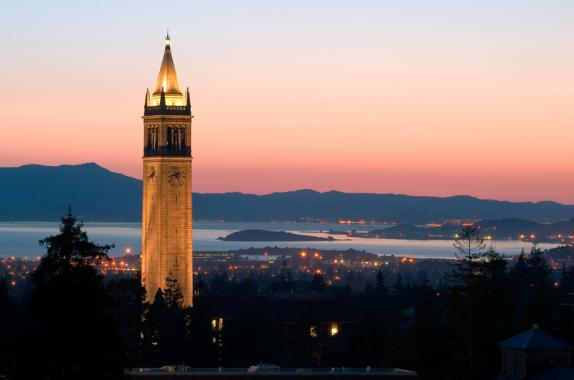
\includegraphics[width=1in]{campanile.jpg}	
	\caption{Berkeley 1}\label{fig:2a}			
\end{subfigure}
\begin{subfigure}[t]{1in}
	\centering
	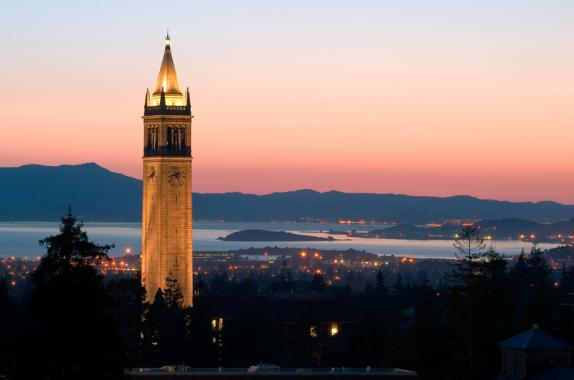
\includegraphics[width=1in]{campanile.jpg}
	\caption{Berkeley 2}\label{fig:2b}		
\end{subfigure}
\end{figure}

In this figure, we have three separate references: one to the overall figure (Figure \ref{fig:2}), one to the first panel (Figure \ref{fig:2a}) and one to the second panel (Figure \ref{fig:2b}). Notice also that instead of specifying the width relative to the text, we gave an explicit width in inches.

\section{Other uses for \LaTeX}

\LaTeX\ isn't actually the only use for its language. It's popularity has generated all kinds of other places it can be used, include a \href{https://chrome.google.com/webstore/detail/tex-for-gmail-inbox/gjnmclkoadjdljnfmbnnhaahilafoeji?hl=en}{plug-in for gmail}. You can even switch Word's input math mode into \LaTeX\ math. In my word documents, when I type \LaTeX\ math symbols into my equations, I actually get the symbols. This is a great, although it doesn't fix how slow Word gets when you include multiple equations.

In the next workshop, we'll talk about other features and uses of \LaTeX\ including tables, footnotes and references/bibliographies, automating exporting from Stata/R to \LaTeX\ and making presentation with \LaTeX.

\section{Resources for further study}

There are a ton of ``getting started in \LaTeX'' resources:
\begin{itemize}
	\item \href{http://www.andy-roberts.net/writing/latex}{Getting to Grips with LaTeX}
	\item \href{ftp://ctan.tug.org/tex-archive/info/lshort/english/lshort.pdf}{The Not So Short Introduction to LaTeX 2$\epsilon$}
	\item \href{https://www.ctan.org/starter}{CTAN's Starting Out in LaTeX Guide}
\end{itemize}

\clearpage
\appendix
\section{Useful packages}

There are a number of useful packages in \LaTeX. Here are the packages we use in the Fundamentals workshop series:
\begin{itemize}
	\item soul: \hl{highlighting}
	\item appendix with \[toc, page\]: lets us make an appendix
	\item enumitem: this package lets us customize list types
	\item amsmath: this package will let us use the align environment, and generally make our equations prettier
	\item hyperref: lets you embed hyperlinks into your document
	\item booktabs: one of the best packages for table formatting
	\item array: lets us create fixed width cells
	\item graphicx: a great package for adding figueres 
	\item caption: for making subcaptions in figures
	\item subcaption: for making subcaptions in figures
	\item dcolumn: required for stargazer
	\item natbib: for making our citations nice
\end{itemize}
We can't cover all of them today, so here are a few others that you might be interested in:
\begin{itemize}
	\item tikzpicture: lets you draw lines and geometric shapes within a TeX document. See \href{http://cremeronline.com/LaTeX/minimaltikz.pdf}{this link}
	\item fancyhdr: lets you add custom headers and footers into your LaTeX document. See \href{https://www.ctan.org/pkg/fancyhdr}{this link}
	\item pdfpages: lets you include pdfs into your TeX document. See \href{https://www.ctan.org/pkg/pdfpages}{this link}
	\item tabularx: lets you create tables that are the same width as the text. There are subtle differences between how tabular, tabular*, and tabularx handle spacing within tables; \href{https://tex.stackexchange.com/questions/341205/what-is-the-difference-between-tabular-tabular-and-tabularx-environments/341212}{this stackexchange} has some helpful examples.
	\item xspace: creates spaces after commands (like \LaTeX); you can use xspace in creating commands to insert that extra space
	\item bibtex and biblatex: both are alternatives to natbib which contain other options for formatting. \href{https://www.sharelatex.com/learn/Bibliography_management_in_LaTeX}{This page} on bibliography management in \LaTeX\ is a great resource.
	\item geometry: lets you customize header, footer and margin width in your document. See \href{https://www.ctan.org/pkg/geometry}{this link}
\end{itemize}

\section{Useful symbols}

All predefined mathematical symbols in \LaTeX\ are available \href{https://oeis.org/wiki/List_of_LaTeX_mathematical_symbols}{here}. An incredibly comprehensive list of 2,590 symbols with the necessary packages and commands is available \href{https://math.uoregon.edu/wp-content/uploads/2014/12/compsymb-1qyb3zd.pdf}{here}. The second link also discuss amsmath extensively.

\section{Templates}

\href{https://www.overleaf.com/latex/templates/}{Overleaf} has a great database of \LaTeX\ templates.

\end{document}